\usetikzlibrary{shapes,arrows}
    \usetikzlibrary{positioning}
    
\begin{figure} [H]
    \centering
    \tikzstyle{frame} = [
        rectangle, draw, 
        text width=4em, text centered,
        minimum height=4em
    ]
    \tikzstyle{line} = [draw, -latex']
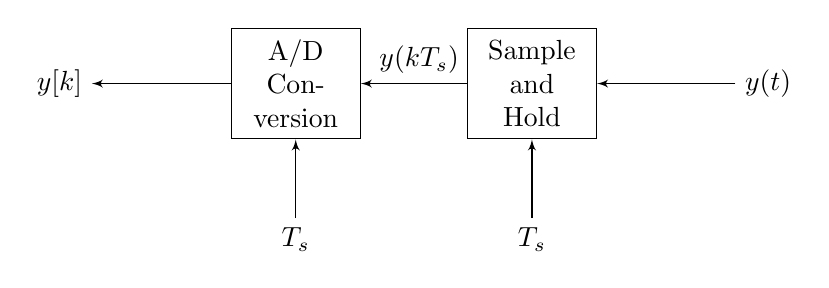
\begin{tikzpicture}[node distance = 3cm]
    \node [frame] (A/D) {A/D Conversion};
    \node [left of=A/D] (yk) {$y[k]$};
    \node [frame, right of=A/D] (SH)  {Sample and Hold};
    \node [right of=SH] (yt)  {$y(t)$};
    \node [below=1cm of SH] (ts)  {$T_s$};
    \node [below=1cm of A/D] (TS)  {$T_s$};

    \path [line] (A/D) -- (yk);
    \path [line] (SH) -- node[above,pos=.45] {$y(kT_s)$} (A/D);
    \path [line] (yt) -- (SH);
    \path [line] (ts) -- (SH);
    \path [line] (TS) -- (A/D);
\end{tikzpicture}
    \caption{A figure of the analog to digital converter....} 
    \label{fig:SH_ADC}
\end{figure}